\documentclass[11pt]{article}
\usepackage[utf8]{inputenc}
\usepackage[spanish,es-tabla]{babel}
\usepackage{amsmath,cancel}
\usepackage{amsfonts}
\usepackage{amssymb}
\usepackage{listings}
\usepackage{xcolor}
\usepackage{tabularx}
\usepackage{adjustbox}
\spanishdecimal{.}
\usepackage{graphicx}
\usepackage{float}
\usepackage[lmargin=2.5cm,rmargin=2.5cm,top=2.5cm,
bottom=2cm]{geometry}
\newcommand{\nombre}{Oscar}
\newcommand{\fecha}{9 de mayo del 2026}
\newcommand{\tituloPractica}{}
%%%%%%%%%%%%%%%%%%%%%%%%%%%%%%%%%%%%%%%%%%%%%%
\begin{document}
\begin{titlepage}
\begin{center}
\vspace*{2\baselineskip}
\hrule height 3pt
\vspace*{0.5\baselineskip}
{\Large \textbf{UNIVERSIDAD DE GUADALAJARA}}\\[0.1cm]
{\large \textbf{CENTRO UNIVERSITARIO DE CIENCIAS EXACTAS E INGENIER\'IAS}}
\vspace*{0.5\baselineskip}
\hrule
\vspace*{3\baselineskip}
\includegraphics[width=0.2\textwidth]{udg}
\vspace*{2\baselineskip}\\
{\large\textbf{ Algor\'itmos Bio-Inspirados \\ Msc. Rob\'otica e Inteligencia Artificial}
\vspace*{\baselineskip}\\
{\large Algoritmo 7 --- Algoritmo Firefly N-Dimensional \vspace{1cm} \\
\begin{tabular}{p{4cm}p{8cm}}
\hline \hline
Nombre del alumno:  & Oscar Alberto Gallo Garc\'ia \\
C\'odigo del alumno:  & 218357704 \\
Profesor: & Dr. Carlos Alberto Lopez Franco \\
 \hline \hline
\end{tabular}
\vfill
\fecha
\end{center}
\newpage
\end{titlepage}

\tableofcontents
\newpage

\section{Resumen}

Se implement\'o el Algoritmo Firefly (FA) para optimizaci\'on continua en $n$ dimensiones. El m\'etodo modela el comportamiento de atracci\'on lumines\-cente entre luci\'ernagas: cada agente se mueve hacia soluciones con mayor brillo (mejor aptitud), con una atracci\'on que decrece en funci\'on de la distancia euclidiana al cuadrado. Se evaluaron doce casos: minimizaci\'on y maximizaci\'on en 2 dimensiones con gr\'aficas de superficie y contorno, y minimizaci\'on y maximizaci\'on en 4 dimensiones.

\section{Metodolog\'ia}

El Algoritmo Firefly fue propuesto por Xin-She Yang en 2008. Est\'a inspirado en el comportamiento de las luci\'ernagas, cuya luz sirve como se\~nal de comunicaci\'on y atracci\'on. En el contexto de optimizaci\'on, el brillo de cada luci\'ernaga es proporcional a su aptitud, y las luci\'ernagas menos brillantes son atra\'idas hacia las m\'as brillantes.

\subsection{Brillo y atractividad}

El brillo de una luci\'ernaga $i$ es directamente proporcional al valor de la funci\'on objetivo $f(\mathbf{x}_i)$: menor $f$ corresponde a mayor brillo en minimizaci\'on, y mayor $f$ en maximizaci\'on.

La atractividad entre dos luci\'ernagas decrece con la distancia euclidiana al cuadrado $r_{ij}^2 = \|\mathbf{x}_i - \mathbf{x}_j\|^2$:

\[
\beta(r_{ij}) = \beta_0 \, e^{-\gamma \, r_{ij}^2}
\]

donde $\beta_0$ es la atractividad m\'axima (en $r=0$) y $\gamma$ es el coeficiente de absorci\'on de luz que controla la velocidad con que $\beta$ decae con la distancia.

\subsection{Ecuaci\'on de movimiento}

Si la luci\'ernaga $j$ es m\'as brillante que $i$, entonces $i$ se mueve hacia $j$ de acuerdo con:

\[
\mathbf{x}_i \leftarrow \mathbf{x}_i + \beta_0 e^{-\gamma r_{ij}^2}(\mathbf{x}_j - \mathbf{x}_i) + \alpha \left(u - \tfrac{1}{2}\right)
\]

donde $u \sim \mathcal{U}(0,1)$ y $\alpha$ es el par\'ametro de aleatoriedad que permite exploraci\'on. Despu\'es de cada movimiento, la posici\'on se proyecta al interior de los l\'imites del dominio.

\subsection{Algoritmo Firefly}

\begin{enumerate}
    \item Inicializar: $\mathbf{x}_i \sim \mathcal{U}(\ell_{\min}, \ell_{\max})^n$ para $i = 1,\ldots,n_p$.
    \item Evaluar $f(\mathbf{x}_i)$ para toda la poblaci\'on.
    \item Repetir hasta $t_{\max}$ iteraciones:
    \begin{enumerate}
        \item Para cada par $(i, j)$: si $j$ es m\'as brillante que $i$, mover $i$ hacia $j$ con la ecuaci\'on de movimiento y proyectar al dominio.
        \item Reevaluar $f(\mathbf{x}_i)$ tras el movimiento.
    \end{enumerate}
    \item Retornar la posici\'on de la luci\'ernaga con mejor aptitud.
\end{enumerate}

\subsection{Par\'ametros}

\begin{table}[H]
\centering
\begin{tabular}{lcc}
\hline\hline
Par\'ametro & 2D & 4D \\
\hline
$\alpha$ (aleatoriedad)              & 0.2  & 0.2  \\
$\beta_0$ (atractividad m\'axima)   & 1.0  & 1.0  \\
$\gamma$ (absorci\'on de luz)       & 1.0  & 1.0  \\
$n_p$ (tama\~no de poblaci\'on)     & 40   & 80   \\
Iteraciones m\'aximas $t_{\max}$    & 200  & 500  \\
\hline\hline
\end{tabular}
\caption{Par\'ametros utilizados en todos los experimentos.}
\end{table}

\subsection{Funciones de prueba}

\begin{align}
f_{\text{esfera}}(\mathbf{x}) &= \sum_{j=1}^{n} x_j^2 \notag\\[4pt]
f_{\text{rastrigin}}(\mathbf{x}) &= 10n + \sum_{j=1}^{n}\bigl[x_j^2 - 10\cos(2\pi x_j)\bigr] \notag\\[4pt]
f_{\text{rosenbrock}}(\mathbf{x}) &= \sum_{j=1}^{n-1}\bigl[100(x_{j+1}-x_j^2)^2 + (1-x_j)^2\bigr] \notag\\[4pt]
f_{\text{ackley}}(\mathbf{x}) &= -20\exp\!\left(-0.2\sqrt{\tfrac{1}{n}\sum x_j^2}\right) - \exp\!\left(\tfrac{1}{n}\sum\cos(2\pi x_j)\right) + 20 + e \notag\\[4pt]
f_{\text{seno-coseno}}(\mathbf{x}) &= \sin(x_1)\cos(x_2) \notag\\[4pt]
f_{\text{easom}}(\mathbf{x}) &= \cos(x_1)\cos(x_2)\exp\!\bigl[-(x_1-\pi)^2-(x_2-\pi)^2\bigr] \notag
\end{align}

\section{Resultados}

\subsection{Minimizaci\'on 2D}

\subsubsection{Funci\'on Esfera}

M\'inimo global en $\mathbf{x}^* = (0,0)$ con $f(\mathbf{x}^*) = 0$. El FA converge con alta precisi\'on: mejor soluci\'on $(1.8\times10^{-4},\,7\times10^{-5})$, $f = 3.59\times10^{-8}$.

\begin{figure}[H]
\centering
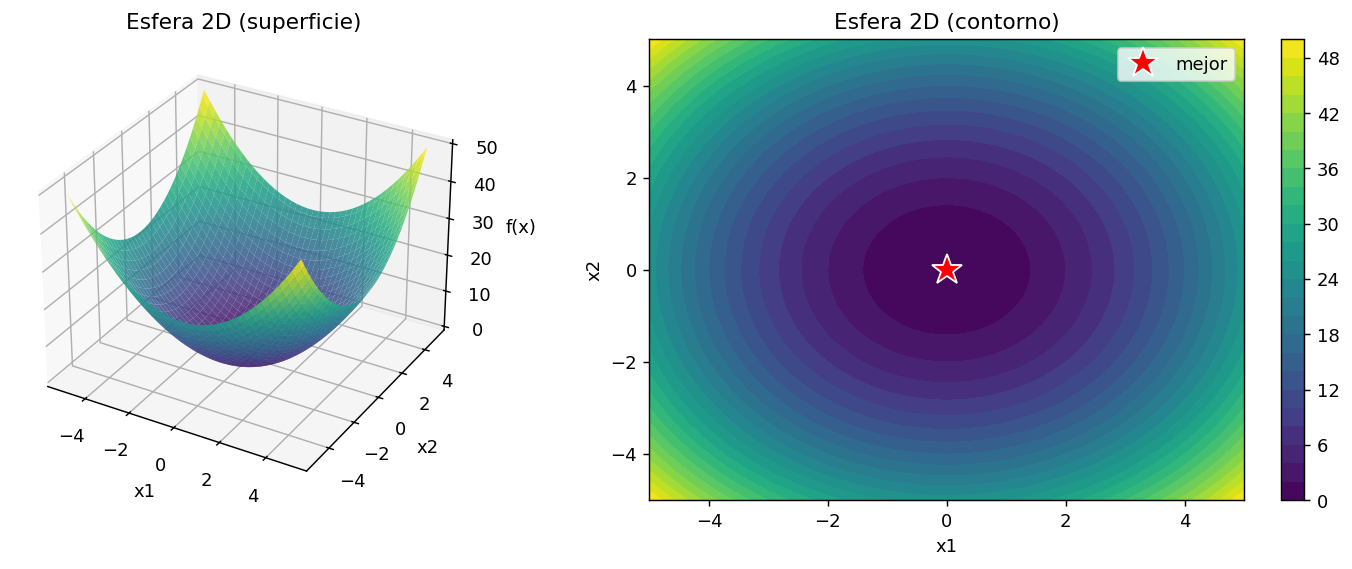
\includegraphics[width=14cm]{figs/FA_min_esfera.png}
\caption{Minimizaci\'on de la funci\'on Esfera. La estrella roja marca la mejor soluci\'on encontrada por el FA.}
\end{figure}

\subsubsection{Funci\'on de Rastrigin}

Funci\'on altamente multimodal con m\'inimo global en $\mathbf{x}^* = (0,0)$, $f = 0$. La alta densidad de m\'inimos locales dificulta la exploraci\'on; el FA queda atrapado en un m\'inimo local: mejor soluci\'on $(1.42\times10^{-3},\,-1.98958)$, $f = 3.98$.

\begin{figure}[H]
\centering
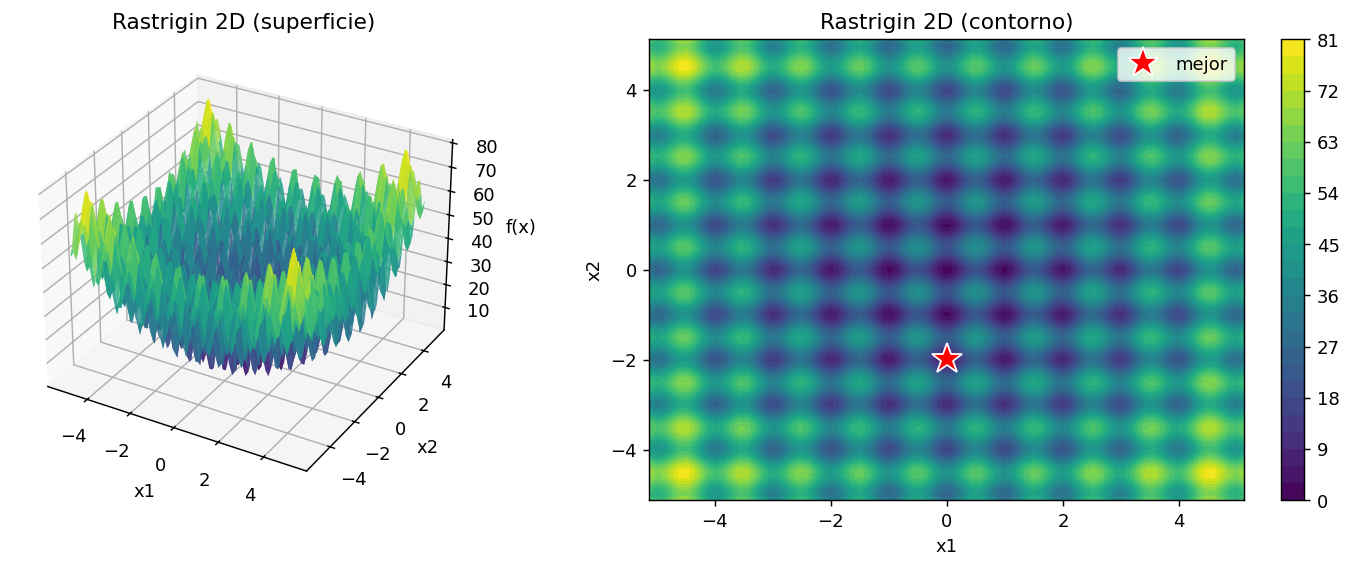
\includegraphics[width=14cm]{figs/FA_min_rastrigin.png}
\caption{Minimizaci\'on de la funci\'on de Rastrigin. La topolog\'ia de valles peri\'odicos propicia la convergencia prematura hacia m\'inimos locales.}
\end{figure}

\subsubsection{Funci\'on de Rosenbrock}

Valle curvo estrecho con m\'inimo global en $\mathbf{x}^* = (1,1)$. El FA sigue correctamente el valle: mejor soluci\'on $(0.99965,\,0.99931)$, $f = 1.36\times10^{-7}$.

\begin{figure}[H]
\centering
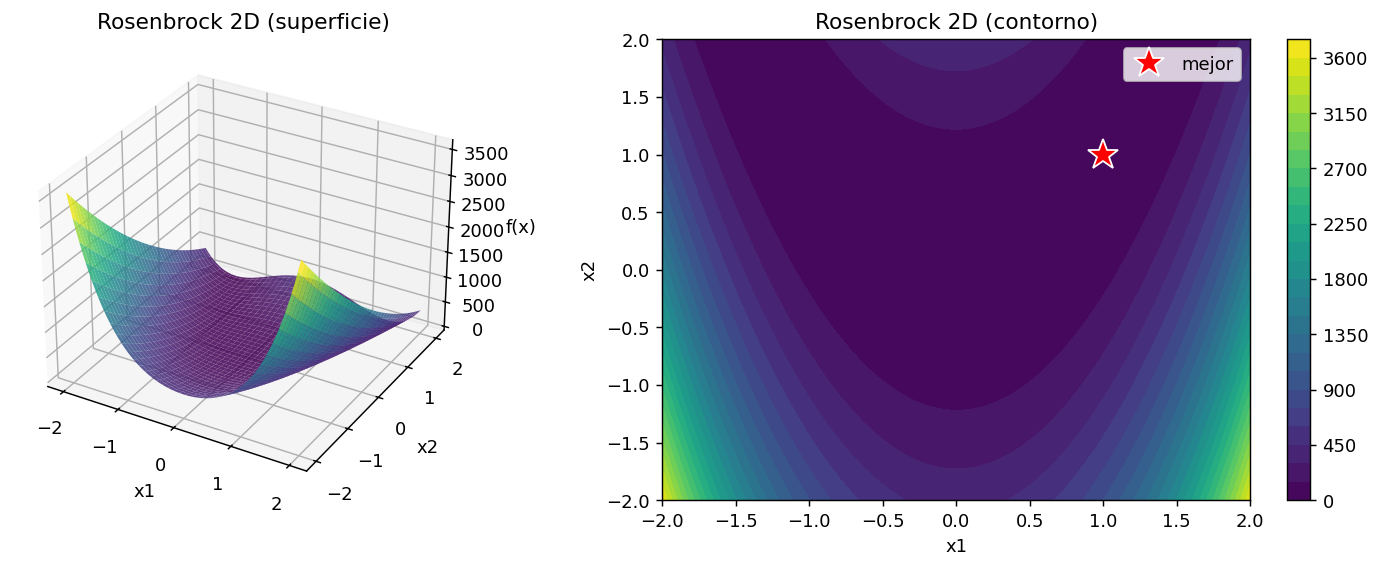
\includegraphics[width=14cm]{figs/FA_min_rosenbrock.png}
\caption{Minimizaci\'on de la funci\'on de Rosenbrock. A pesar del valle estrecho y curvo, la atracci\'on entre luci\'ernagas dirige la poblaci\'on hacia el m\'inimo.}
\end{figure}

\subsection{Maximizaci\'on 2D}

\subsubsection{Esfera Negativa}

Se maximiza $-f_{\text{esfera}}(\mathbf{x})$, cuyo m\'aximo global es en $(0,0)$ con valor $0$. Mejor soluci\'on $(-8\times10^{-5},\,1.5\times10^{-4})$, $f = -2.97\times10^{-8}$.

\begin{figure}[H]
\centering
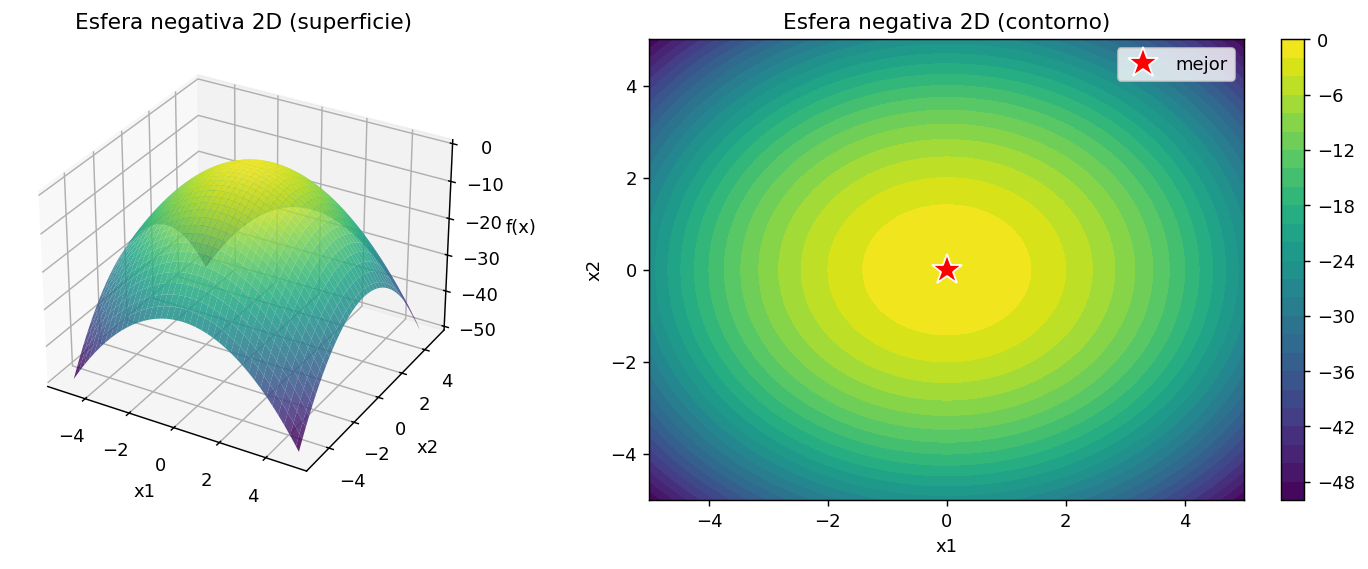
\includegraphics[width=14cm]{figs/FA_max_neg_esfera.png}
\caption{Maximizaci\'on de la esfera negativa. La poblaci\'on converge al v\'ertice de la par\'abola invertida.}
\end{figure}

\subsubsection{Funci\'on Seno-Coseno}

$f = \sin(x_1)\cos(x_2)$ tiene m\'ultiples m\'aximos globales de valor $1.0$; entre ellos $(-\pi/2,\,\pi)$. El FA localiza uno: mejor soluci\'on $(-1.5708,\,3.14159)$, $f \approx 1.0$.

\begin{figure}[H]
\centering
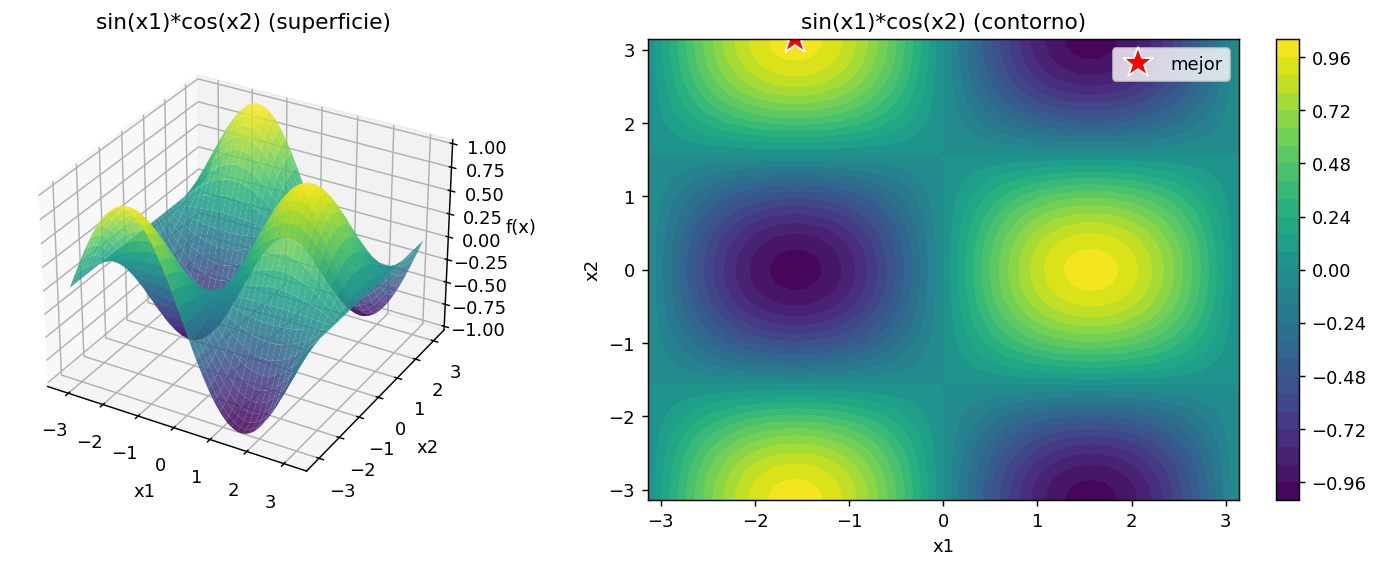
\includegraphics[width=14cm]{figs/FA_max_seno_coseno.png}
\caption{Maximizaci\'on de $\sin(x_1)\cos(x_2)$. La funci\'on presenta m\'ultiples m\'aximos id\'enticos; el FA localiza uno de ellos con valor $f \approx 1$.}
\end{figure}

\subsubsection{Funci\'on Easom}

M\'aximo global en $(\pi,\,\pi)$ con $f = 1.0$. La funci\'on es casi cero fuera de un pico muy estrecho. El FA lo localiza con alta precisi\'on: mejor soluci\'on $(3.14159,\,3.14118)$, $f = 0.99999974$.

\begin{figure}[H]
\centering
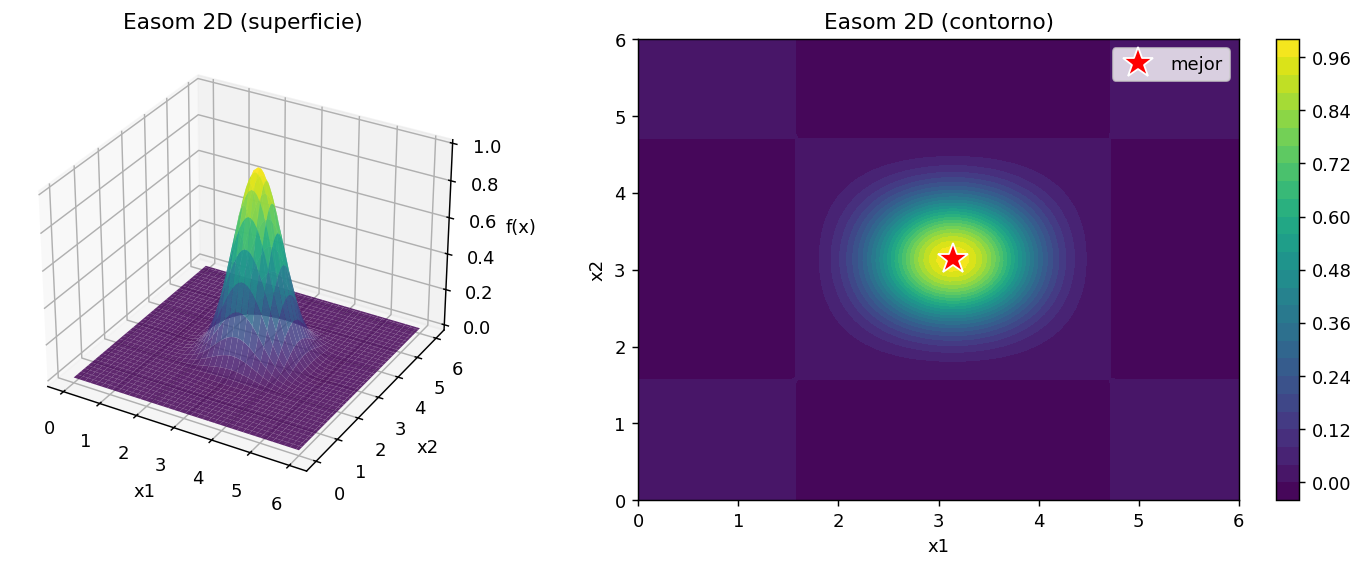
\includegraphics[width=14cm]{figs/FA_max_easom.png}
\caption{Maximizaci\'on de Easom. La atracci\'on de luci\'ernagas concentra la poblaci\'on en el pico estrecho de $(\pi,\pi)$.}
\end{figure}

\subsection{Minimizaci\'on N-Dimensional (4D)}

\begin{table}[H]
\centering
\begin{tabular}{lp{8.5cm}r}
\hline\hline
Funci\'on & Mejor soluci\'on & $f(\hat{\mathbf{x}})$ \\
\hline
Esfera    & $[-6.4{\times}10^{-4},\;1.09{\times}10^{-3},\;-1.62{\times}10^{-3},\;1.22{\times}10^{-3}]$ & $5.72\times10^{-6}$ \\[3pt]
Rastrigin & $[0.99449,\;-0.99947,\;-5.36{\times}10^{-3},\;-0.9951]$ & $2.99$ \\[3pt]
Ackley    & $[6.10377,\;0.86354,\;-2.89565,\;4.96029]$ & $11.87$ \\
\hline\hline
\end{tabular}
\caption{Resultados de minimizaci\'on en 4 dimensiones. Esfera converge al \'optimo global; Rastrigin y Ackley quedan en m\'inimos locales.}
\end{table}

\subsection{Maximizaci\'on N-Dimensional (4D)}

Se maximizan las versiones negadas de las funciones anteriores.

\begin{table}[H]
\centering
\begin{tabular}{lp{8.5cm}r}
\hline\hline
Funci\'on & Mejor soluci\'on & $f(\hat{\mathbf{x}})$ \\
\hline
$-$Esfera    & $[8.6{\times}10^{-4},\;-1.3{\times}10^{-4},\;2.06{\times}10^{-3},\;-5.16{\times}10^{-3}]$ & $-3.16\times10^{-5}$ \\[3pt]
$-$Rastrigin & $[-0.99565,\;1.45{\times}10^{-3},\;-2.1{\times}10^{-3},\;1.99035]$ & $-4.98$ \\[3pt]
$-$Ackley    & $[-3.10775,\;-12.71153,\;6.85589,\;6.03334]$ & $-16.96$ \\
\hline\hline
\end{tabular}
\caption{Resultados de maximizaci\'on en 4 dimensiones. El comportamiento es sim\'etrico al de minimizaci\'on: Esfera converge, Rastrigin y Ackley permanecen en \'optimos locales.}
\end{table}

\section{Conclusi\'on}

El Algoritmo Firefly demostr\'o ser efectivo en funciones unimodales y suaves: la Esfera convergi\'o al \'optimo global tanto en 2D como en 4D con errores del orden de $10^{-6}$, y Rosenbrock localiz\'o el valle estrecho con $f \approx 1.4\times10^{-7}$. En maximizaci\'on 2D, las funciones Seno-Coseno y Easom alcanzaron valores muy cercanos a $1.0$, lo que confirma la capacidad del algoritmo para localizar picos angostos.\\\\
La principal limitaci\'on observada fue la convergencia prematura en funciones altamente multimodales. Rastrigin atrap\'o la poblaci\'on en m\'inimos locales de periodo $1$ en 2D y 4D, mientras que Ackley en 4D con dominio $[-32,32]$ present\'o el peor desempe\~no ($f \approx 11.87$). Esto se debe a que el coeficiente $\gamma = 1.0$ provoca que la atractividad decaiga muy r\'apidamente para distancias grandes, reduciendo el alcance efectivo de la exploraci\'on global en dominios amplios.\\\\
El par\'ametro $\alpha$ controla el equilibrio entre exploraci\'on y explotaci\'on: valores mayores favorecen la diversidad pero retardan la convergencia, mientras que valores peque\~nos aceleran la convergencia local. Para Rastrigin y Ackley en espacios de alta dimensi\'on ser\'ia recomendable reducir $\gamma$ (mayor alcance de atracci\'on) o usar un esquema adaptativo de $\alpha$ que disminuya a lo largo de las iteraciones.

\end{document}
